%%%%%%%%%%%%%%%%%%%%%%%%%%%%%%%%%%%%%%%%%%%%%%%%%%%%%%%%%%%%%%%%%%%%%%%%%%%%%%%%
%%
%%   BornAgain User Manual
%%
%%   homepage:   http://www.bornagainproject.org
%%
%%   copyright:  Forschungszentrum Jülich GmbH 2015
%%
%%   license:    Creative Commons CC-BY-SA
%%   
%%   authors:    Scientific Computing Group at MLZ Garching
%%               C. Durniak, M. Ganeva, G. Pospelov, W. Van Herck, J. Wuttke
%%
%%%%%%%%%%%%%%%%%%%%%%%%%%%%%%%%%%%%%%%%%%%%%%%%%%%%%%%%%%%%%%%%%%%%%%%%%%%%%%%%


\newpage
\chapter{Using the Python API}  \SecLabel{Usage}


%%%%%%%%%%%%%%%%%%%%%%%%%%%%%%%%%%%%%%%%%%%%%%%%%%%%%%%%%%%%%%%%%%%%%%%%%%%%%%%%
\section{Running a simulation}
%%%%%%%%%%%%%%%%%%%%%%%%%%%%%%%%%%%%%%%%%%%%%%%%%%%%%%%%%%%%%%%%%%%%%%%%%%%%%%%%

A simulation of GISAS using \BornAgain\ consists of the following steps:
\begin{itemize}
\item define materials by specifying name and refractive index,
\item define layers by specifying thickness, roughness, material,
\item define embedded particles by specifying shape, size,
   constituting material, interference function,
\item embed the particles in layers, specifying density, position, orientation, 
\item assemble a multilayered sample,
\item specify input beam and detector characteristics,
\item run the simulation,
\item save the simulated detector image.
\end{itemize}

\noindent
All these steps can be organized in either a Graphical User Interface (GUI) or by providing a Python script with the simulation description. 
In the following, we describe how to write a 
\Code{Python} script which runs a \BornAgain\ simulation. For tutorials about this programming language, the users are referred to \cite{Lut09}.


% More information about the general software architecture and \BornAgain\ internal design are given in \SecRef{SoftwareArchitecture}.


%===============================================================================
\subsection{Units:} 
%===============================================================================
\index{Units}

By default the angles are expressed in radians and the lengths are given in
nanometers.  But it is possible to use other units by
specifying them right after the value of the corresponding
parameter like, for example, \Code{20.0*micrometer}.


%===============================================================================
\subsection{A first example} \SecLabel{Example1Python}
%===============================================================================

In this example, we simulate the scattering from a mixture of
cylindrical and prismatic nanoparticles without any interference
between them. These particles are placed in air, on top
of a substrate.\\ We are going to go through each step of the
simulation. The \Python\ code snippet specific to each stage will be given at
the beginning of the description. 
More examples can be found at our project web site \url{http://www.bornagainproject.org/documentation/python_examples}

% But for the sake of completeness the full code is given
% in Appendix~\ref{PythonSimulationExampleScript}.

%-------------------------------------------------------------------------------
\subsubsection{Importing Python modules}
%-------------------------------------------------------------------------------

\begin{lstlisting}[language=python, style=eclipseboxed,name=ex1,nolol]
import numpy @\label{import_lib_beg}@
import matplotlib
import pylab @\label{import_lib_end}@
from bornagain import * @\label{import_ba}@
\end{lstlisting}
We start by importing different functions from external
modules, for example \Code{NumPy} (lines~\ref{import_lib_beg}-\ref{import_lib_end}), which
is a fundamental package for scientific computing with \Python\
\cite{s:numpy}.  In particular, line~\ref{import_ba}
imports the features of \BornAgain\ software.

%-------------------------------------------------------------------------------
\subsubsection{Defining the materials} 
%-------------------------------------------------------------------------------

\begin{lstlisting}[language=python, style=eclipseboxed,name=ex1,nolol]
def get_sample(): @\label{def_function}@
    """
    Build and return the sample representing cylinders and pyramids on top of substrate without interference.
   """
    # defining materials @\label{material1}@
    m_air = HomogeneousMaterial("Air", 0.0, 0.0)  @\label{material2}@
    m_substrate = HomogeneousMaterial("Substrate", 6e-6, 2e-8) @\label{material3}@
    m_particle = HomogeneousMaterial("Particle", 6e-4, 2e-8) @\label{materialparticle}@

\end{lstlisting}
Line~\ref{def_function} marks the beginning of the
function to define our sample. Lines~\ref{material2}, \ref{material3} and \ref{materialparticle} define different
materials using class \Code{HomogeneousMaterial}. The general syntax is the following 
\begin{lstlisting}[language=python, style=eclipse,numbers=none]
<material_name> = HomogeneousMaterial("name", delta, beta)
\end{lstlisting}
where \Code{name} is the name of the
material associated with its complex refractive index
n=1-\Code{delta} +i \Code{beta}. \Code{<material\_name>} is later used when
referring to this particular material. The three materials defined in this example are \Code{Air} with a refractive
index of 1 (\Code{delta = beta = 0}), a \Code{Substrate} associated with a complex refractive index
equal to $1-6\times 10^{-6} +i2\times 10^{-8} $, and the material of the particles, whose refractive index is \Code{n}$=1-6\times 10^{-4}+i2\times 10^{-8}$.

%-------------------------------------------------------------------------------
\subsubsection{Defining the particles}
%-------------------------------------------------------------------------------
\begin{lstlisting}[language=python,style=eclipseboxed,name=ex1,nolol]
    # collection of particles @\label{particles1}@
    cylinder_ff = FormFactorCylinder(5*nanometer, 5*nanometer) @\label{particlescyl1}@
    cylinder = Particle(m_particle, cylinder_ff) @\label{particlescyl2}@
    prism_ff = FormFactorPrism3(10*nanometer, 5*nanometer) @\label{particlesprism1}@
    prism = Particle(m_particle, prism_ff) @\label{particlesprism2}@
\end{lstlisting}
We implement two different shapes of particles: cylinders and
prisms (\textit{i.e.} elongated particles with a constant equilateral triangular cross section).
 
All particles implemented in \BornAgain\ are defined by their
form factors (see Appendix~\ref{app:ff}), their sizes and the material
they are made of. Here, for the
cylindrical particle, we input its radius and height.  For the prism, 
the possible inputs are the length of one side of its equilateral triangular
base and its height.

In order to define a particle, we proceed in two steps. For example for
the cylindrical particle, we first specify the form factor of a cylinder with 
its radius and height, both equal to 5 nanometers in this particular
case (see line~\ref{particlescyl1}). Then we associate this shape with
the constituting material as in line~\ref{particlescyl2}.
The same procedure has been applied for the prism in lines~\ref{particlesprism1} and \ref{particlesprism2}, respectively.

%-------------------------------------------------------------------------------
\subsubsection{Characterizing particles assembly} 
%-------------------------------------------------------------------------------
\begin{lstlisting}[language=python, style=eclipseboxed, name=ex1,nolol]
    particle_layout = ParticleLayout()  @\label{particlesdecor1}@
    particle_layout.addParticle(cylinder, 0.0, 0.5)  @\label{particlesdecor2}@
    particle_layout.addParticle(prism, 0.0, 0.5)@\label{particlesdecor3}@
    interference = InterferenceFunctionNone()  @\label{particlesnointerf}@
    particle_layout.addInterferenceFunction(interference)  @\label{particlesinterf}@
\end{lstlisting}
The object which holds the information about the positions and densities of particles
in our sample is called \Code{ParticleLayout}
(line~\ref{particlesdecor1}). We use the associated function \Code{addParticle}
for each particle shape (lines~\ref{particlesdecor2}, \ref{particlesdecor3}). Its general syntax is 

\begin{lstlisting}[language=python, style=eclipse,numbers=none]
addParticle(<particle_name>, depth, abundance) 
\end{lstlisting}
where \Code{<particle\_name>} is the name used to define the particles
(lines~\ref{particlescyl2} and \ref{particlesprism2}), \Code{depth}
(default value = 0)
is the vertical position, expressed in nanometers, of the particles in a given layer (the
association with a particular layer will be done during the next step) and
\Code{abundance} is the proportion of this type of particles, 
normalized to the total number of particles. Here we have 50\% of cylinders
and 50\% of prisms.

\ImportantPoint{Remark:}{Depth of particles\\
The vertical positions of the particles in a layer are given in relative
coordinates. For the top layer, the bottom of the layer corresponds to
\Code{depth}=0 and negative values would correspond to particles
floating above layer 1 since the vertical axis, shown in \reffig{multil3d} is pointing upwards. But for all the other layers, it is the top of the
layer which corresponds to \Code{depth}=0.}\\


\noindent Finally, lines~\ref{particlesnointerf} and
\ref{particlesinterf} specify that there is \textbf{no coherent interference} between
the waves scattered by these particles. In this case, the intensity is calculated by
the incoherent sum of the scattered waves: $\langle |F_j|^2\rangle$,
where $F_j$ is the form factor associated with the particle of type $j$.  The way these waves
interfere imposes the horizontal distribution of
the particles as
the interference reflects the long or short-range order of the
particles distribution (see  \SecRef{sect:interf}). On the contrary, the vertical position is
imposed when we add the particles in a given layer by parameter \Code{depth}, as shown in lines~\ref{particlesdecor2} and \ref{particlesdecor3}.

%-------------------------------------------------------------------------------
\subsubsection{Multilayer}
%-------------------------------------------------------------------------------
\begin{lstlisting}[language=python, style=eclipseboxed,name=ex1,nolol]
# air layer with particles and substrate form multi layer  @\label{sampleassembling}@
    air_layer = Layer(m_air) @\label{airlayer}@
    air_layer.addLayout(particle_layout) @\label{airlayerdecorator}@
    substrate_layer = Layer(m_substrate, 0)  @\label{substratelayer}@
    multi_layer = MultiLayer() @\label{multilayercanvas}@
    multi_layer.addLayer(air_layer) @\label{layerairdecor}@
    multi_layer.addLayer(substrate_layer) @\label{layersubstrate}@
    return multi_layer @\label{returnmlayer}@
\end{lstlisting}
We now have to configure our sample. For this first example,
the particles, \textit{i.e.} cylinders and prisms, are on top of a substrate in an
air layer. \textbf{The order in which we define these layers is important: we
start from the top layer down to the bottom one}.

Let us start with the air layer. It contains the particles. In
line~\ref{airlayer}, we use the previously defined \Code{m\_air}
(="air" material) (line~\ref{material2}). The command in line~\ref{airlayerdecorator} shows that this layer contains particles
which are defined using particle layout object. The substrate layer
only contains the substrate material (line~\ref{substratelayer}).
%Note that the
%\Code{depth} is referenced to the bottom of the top layer (negative
%values would correspond to particles floating above layer 1 as
%the vertical axis is pointing upwards). 
 
There are different possible syntaxes to define a layer. As shown in
lines~\ref{airlayer} and \ref{substratelayer}, we can use
\Code{Layer(<material\_name>,thickness)} or
\Code{Layer(<material\_name>)}. The second case corresponds
to the default value of the \Code{thickness}, equal to 0. The \Code{thickness} is
expressed in  nanometers.

Our two layers are now fully characterized. The sample is assembled using
\Code{MultiLayer()} constructor (line~\ref{multilayercanvas}): we start with the air layer decorated
with the particles (line~\ref{layerairdecor}), which is the layer at
the top and end with the bottom layer, which is the
substrate (line~\ref{layersubstrate}).

%-------------------------------------------------------------------------------
\subsubsection{Characterizing the input beam and output detector}
%-------------------------------------------------------------------------------

\begin{lstlisting}[language=python, style=eclipseboxed,name=ex1,nolol]
def get_simulation():  @\label{run1}@
    """
    Create and return GISAXS simulation with beam and detector defined
    """
    simulation = Simulation() @\label{run2}@
    simulation.setDetectorParameters(100, -1.0*degree, 1.0*degree, 100, 0.0*degree, 2.0*degree) @\label{rundetector}@
    simulation.setBeamParameters(1.0*angstrom, 0.2*degree, 0.0*degree) @\label{runbeam}@
    return simulation @\label{returnsimul}@
\end{lstlisting}
The first stage is to create the \Code{Simulation()} object (line~\ref{run2}). Then we define the detector (line~\ref{rundetector}) and beam
parameters (line~\ref{runbeam}). %, which are associated with the
%sample previously defined (line~\ref{runsample}). Finally we run
%the simulation (line~\ref{runsimul}). 
Those functions are part of the Simulation
class.  The different incident and exit angles are
shown in \reffig{multil3d}.

The detector parameters are set using ranges of angles via
the function:

\begin{lstlisting}[language=python, style=eclipse,numbers=none]
setDetectorParameters(n_phi, phi_f_min, phi_f_max, n_alpha, alpha_f_min, alpha_f_max),
\end{lstlisting}


\noindent where number of bins \Code{n\_phi}, low edge of first bin \Code{phi\_f\_min} and
upper edge of last bin \Code{phi\_f\_max} all together define $\phi_f$ detector axis, 
while \Code{n\_alpha}, \Code{alpha\_f\_min} and \Code{alpha\_f\_max} are related to 
$\alpha_f$ detector axis.

\ImportantPoint{Remark:}{Axis binning\\
By default axes are binned to provide constant bin size in k-space, which means slightly
non-equidistant binning in angle space. Other possible options, including user defined
axes with custom variable bin size are explained elsewhere.
}
\vspace*{2mm}

%are the minimum and maximum values of $\phi_f$, respectively, \Code{n\_alpha} is
%the number of bins for $\alpha_f$ axis, \Code{alpha\_f\_min} and \Code{alpha\_f\_max} 
%are the minimum and maximum values of
%$\alpha_f$, respectively.

%\Code{isgisaxs\_style=True} (default value = \Code{False}) is a boolean
%used to characterise the structure of the output data. If
%\Code{isgisaxs\_style=True}, the output data is binned at constant
%values of the sine of the output angles, $\alpha_f$ and $\phi_f$, otherwise it is binned
%at constant values of these two angles.\\

\noindent To characterize the beam we use function 
\begin{lstlisting}[language=python, style=eclipse,numbers=none]
setBeamParameters(lambda, alpha_i, phi_i),
\end{lstlisting}

\noindent where \Code{lambda} is the incident beam wavelength,
\Code{alpha\_i} is the incident
grazing angle on the surface of the sample,
\Code{phi\_i} is the in-plane
direction of the incident beam (measured with respect to the $x$-axis).


%-------------------------------------------------------------------------------
\subsubsection{Running the simulation and plotting the results}
%-------------------------------------------------------------------------------

\begin{lstlisting}[language=python, style=eclipseboxed,name=ex1,nolol]
def run_simulation(): @\label{run_simulation}@
    """
   Run simulation and plot results
    """
    sample = get_sample() @\label{get_sample}@
    simulation = get_simulation() @\label{get_simulation}@
    simulation.setSample(sample)  @\label{setsample}@
    simulation.runSimulation()  @\label{runsimul}@
    result = simulation.getIntensityData().getArray() + 1  # for log scale  @\label{outputdata}@
    pylab.imshow(numpy.rot90(result, 1), norm=matplotlib.colors.LogNorm(), extent=[-1.0, 1.0, 0, 2.0]) @\label{plot1}@
    pylab.show() @\label{plot2}@
\end{lstlisting}
%In function \Code{run\_simulation()}, we associate the sample
%characterised by function \Code{get\_sample()} with the input beam and
%output detector, defined in function \Code{get\_simulation()} (line~\ref{runsample}).
The function, whose definition starts from line~\ref{run_simulation}, gathers all
items. We create the sample and the simulation objects at the lines 
~\ref{get_sample} and \ref{get_simulation}, using calls to the previously defined functions. We assign the sample to the simulation at line ~\ref{setsample} and
finally launch the simulation at line ~\ref{runsimul}.

In line~\ref{outputdata} we obtain the simulated intensity
as a function of outgoing angles $\alpha_f$ and $\phi_f$ for further
uses (plots, fits,\ldots) as a \Code{NumPy} array containing
\Code{n\_phi}$\times$\Code{n\_alpha}
datapoints. Lines~\ref{plot1}-\ref{plot2} produces the two-dimensional
contour plot of the intensity as a function of $\alpha_f$ and
$\phi_f$ shown in \reffig{output_ex1}. 

\begin{figure}[htbp]
  \begin{center}
   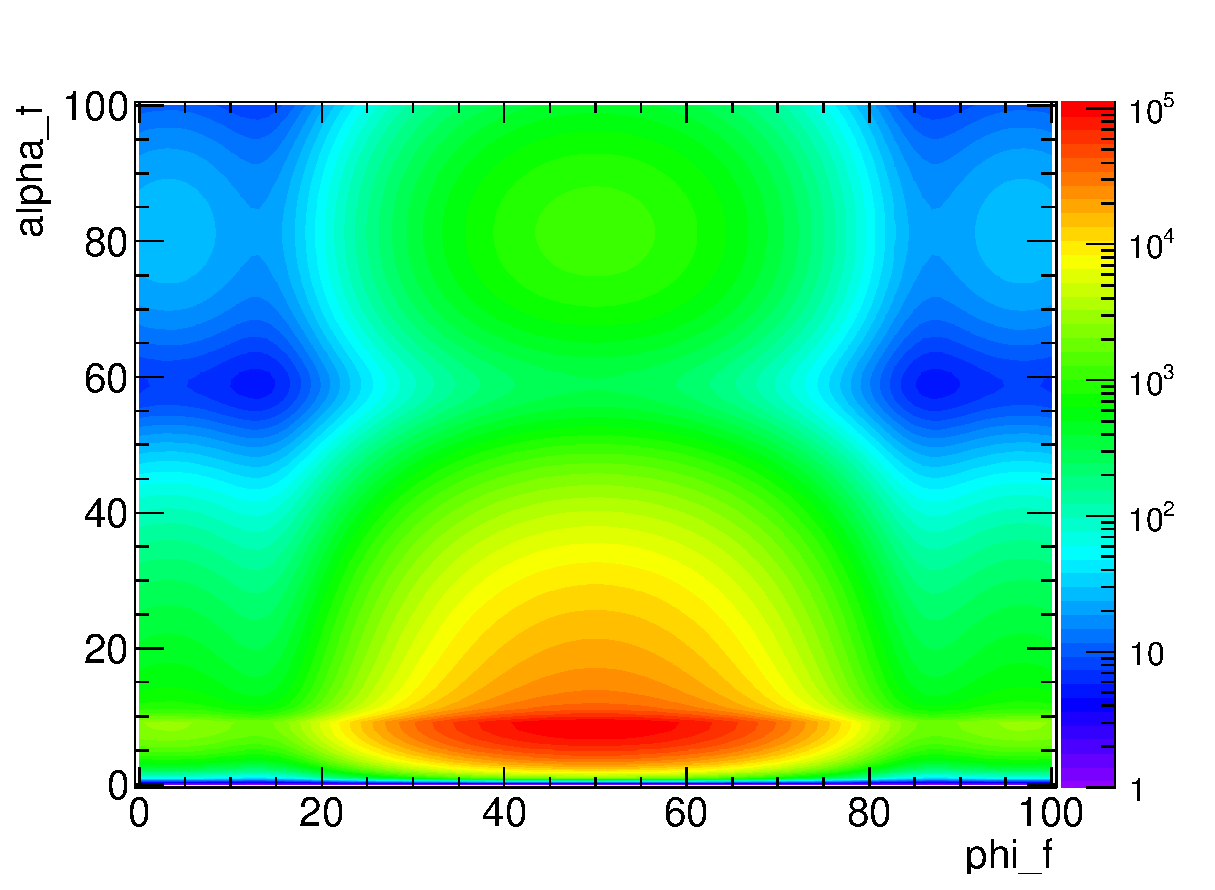
\includegraphics[clip=true, width=120mm]{fig/gisasmap/Manual_ex1.eps}
  \end{center}
  \caption[Example 1: Simulated grazing-incidence small-angle X-ray scattering from a mixture of
cylindrical and prismatic nanoparticles without any interference, deposited on top
of a substrate]{Simulated grazing-incidence small-angle X-ray scattering from a mixture of
cylindrical and prismatic nanoparticles without any interference, deposited on top
of a substrate. The input beam is characterized by a wavelength
$\lambda$ of 1~\AA\ and incident angles $\alpha_i=0.2^{\circ}$, $\phi_i=0^{\circ}$. The
cylinders have a radius and a height both equal to 5~nm, the prisms
are characterized by a side length equal to 10~nm and they are 5~nm high. The
material of the particles has a refractive index of $1-6\times 10^{-4}+i2\times 10^{-8}$. For the substrate
it is equal to $1-6\times 10^{-6} +i2\times 10^{-8} $. The color scale
is associated with the output intensity in arbitrary units. }
\label{fig:output_ex1}
\end{figure}


%===============================================================================
\subsection{Working with sample parameters}
   \SecLabel{WorkingWithSampleParameters}
%===============================================================================


This section gives additional details about the manipulation of sample parameters
during run time; that is after the sample has already been constructed. 
For a single simulation this is normally not necessary. However it might be useful
during interactive work when the user tries to find optimal sample parameters by
running a series of simulations.
A similar task also arises when the theoretical model, composed of the
description of the sample and of the simulation, is used for fitting real data.
In this case, the fitting kernel requires a list of the existing sample parameters
and a mechanism for changing the values of these parameters in order to find 
their optima.

In \BornAgain\ this is done using the so-called sample parameter pool
mechanism. We are going to briefly explain this approach using the example
of \SecRef{Example1Python}.

In \BornAgain\ a sample is described by a hierarchical tree of objects.
For the multilayer created in the previous section this tree can be graphically
represented as shown in Fig.~\ref{fig:sample_tree}. Similar trees can
be printed in a \Python\
session by running \Code{multi\_layer.printSampleTree()}

\begin{figure}[p!]

\tikzstyle{every node}=[draw=black,thick,anchor=west]
\tikzstyle{selected}=[draw=red,fill=red!30]
\tikzstyle{optional}=[dashed,fill=gray!50]
\begin{tikzpicture}[%
  grow via three points={one child at (0.5,-0.7) and
  two children at (0.5,-0.7) and (0.5,-1.4)},
  edge from parent path={(\tikzparentnode.south) |- (\tikzchildnode.west)}]
  \node {MultiLayer}
    child { node {Layer \#0}
		child { node {ParticleLayout } 
			child { node {Particle Info 0} 
				child {node {Particle }  
					child { node {FormFactorCylinder} 
						child { node [optional] { radius:5.0} }					
						child { node [optional] { height:5.0} }					
					}				
				}
    			child [missing] {}		
    			child [missing] {}		
			    child [missing] {}		
				child {node [optional] { abundance:0.5} }			
				child {node [optional] { depth:0.0} }			
			}
    		child [missing] {}		
    		child [missing] {}		
			child [missing] {}		
    		child [missing] {}		
    		child [missing] {}		
			child [missing] {}		
			child { node {Particle Info 1} 
				child {node {Particle }  
					child { node {FormFactorPrism3} 
						child { node [optional] { length:10.0} }					
						child { node [optional] { height:5.0} }					
					}				
				}
    			child [missing] {}		
    			child [missing] {}		
			    child [missing] {}		
				child {node [optional] { abundance:0.5} }			
				child {node [optional] { depth:0.0} }						
			}					
		}
		child [missing] {}		
   		child [missing] {}		
	    child [missing] {}		
		child [missing] {}		
   		child [missing] {}		
	    child [missing] {}		
	    child [missing] {}		
		child [missing] {}		
   		child [missing] {}		
	    child [missing] {}		
		child [missing] {}		
   		child [missing] {}		
	    child [missing] {}		
	    child [missing] {}		
		child {node [optional] { thickness:0.0} }				
    }
	child [missing] {}		
   	child [missing] {}		
	child [missing] {}		
   	child [missing] {}		
	child [missing] {}		
	child [missing] {}		
   	child [missing] {}		
	child [missing] {}		
   	child [missing] {}		
	child [missing] {}		
	child [missing] {}		
   	child [missing] {}		
	child [missing] {}		
   	child [missing] {}		
	child [missing] {}		
	child [missing] {}		
	child { node {Layer interface \#0} 
    	child {node { roughness} 
    		child {node [optional] { corrlength:0.0} }				    	
    		child {node [optional] { hurst:0.0} }				    	
    		child {node [optional] { sigma:0.0} }				    	
    	}					
	}
   	child [missing] {}		
	child [missing] {}		
	child [missing] {}		
    child { node {Layer \#1}
    	child {node [optional] { thickness:0.0} }				
    }
	child [missing] {}		
    child { node [optional] {CrossCorrLength:0.0} };
    
\end{tikzpicture}
\caption{Tree representation of the sample structure.}
\label{fig:sample_tree}
\end{figure}


The top \Code{MultiLayer} object is composed of three children, namely
\Code{Layer \#0, Layer Interface \#0} and \Code{Layer \#1}. The
children objects might themselves also be decomposed into tree-like structures. For example,
\Code{Layer \#0} contains a \Code{ParticleLayout} object, which holds information
related to the two types of particles populating the layer. All numerical values used
during the sample construction (thickness of layers, size of particles, roughness parameters) are part of the same tree structure. 
They are marked in the figure with shaded gray boxes.

These values are registered in the sample parameter pool using the name
composed of the corresponding nodes' names. And they can be accessed/changed
during run time. For example, the \Code{height} of the cylinders
populating the first layer can be changed from the
current value of $5~\rm{nm}$ to $1~\rm{nm}$ by running the command

\begin{lstlisting}[language=shell, style=commandline]
multi_layer.setParameterValue('/MultiLayer/Layer0/ParticleLayout/ParticleInfo0/Particle/FormFactorCylinder/height', 1.0)
\end{lstlisting}


A list of the names and values of all registered sample's parameters
can be displayed using the command 

\begin{lstlisting}[language=shell, style=commandline]
> multi_layer.printParameters()
The sample contains following parameters ('name':value)
'/MultiLayer/Layer0/ParticleLayout/ParticleInfo0/Particle/FormFactorCylinder/height':5
'/MultiLayer/Layer0/ParticleLayout/ParticleInfo0/Particle/FormFactorCylinder/radius':5
'/MultiLayer/Layer0/ParticleLayout/ParticleInfo0/abundance':0.5
'/MultiLayer/Layer0/ParticleLayout/ParticleInfo0/depth':0
'/MultiLayer/Layer0/ParticleLayout/ParticleInfo1/Particle/FormFactorPrism3/length':5
'/MultiLayer/Layer0/ParticleLayout/ParticleInfo1/Particle/FormFactorPrism3/height':5
'/MultiLayer/Layer0/ParticleLayout/ParticleInfo1/abundance':0.5
'/MultiLayer/Layer0/ParticleLayout/ParticleInfo1/depth':0
'/MultiLayer/Layer0/thickness':0
'/MultiLayer/Layer1/thickness':0
'/MultiLayer/LayerInterface/roughness/corrlength':0
'/MultiLayer/LayerInterface/roughness/hurst':0
'/MultiLayer/LayerInterface/roughness/sigma':0
'/MultiLayer/crossCorrLength':0
\end{lstlisting}

Wildcards \Code{'*'} can be used to reduce typing or to work on a group
of parameters. In the example below, the first command will change the
height of all cylinders in the same way, as in the previous example. The second line will change simultaneously the height of {\it both} cylinders and prisms.
\begin{lstlisting}[language=shell, style=commandline]
multi_layer.setParameterValue('*FormFactorCylinder/height', 1.0)
multi_layer.setParameterValue('*height', 1.0)
\end{lstlisting}

The complete example described in this section can be found at 
\begin{lstlisting}[language=shell, style=commandline]
./Examples/python/fitting/ex001_SampleParametersIntro/SampleParametersIntro.py
\end{lstlisting}

%%%%%%%%%%%%%%%%%%%%%%%%%%%%%%%%%%%%%%%%%%%%%%%%%%%%%%%%%%%%%%%%%%%%%%%%%%%%%%%%
\section{Fitting} \SecLabel{Fitting}
%%%%%%%%%%%%%%%%%%%%%%%%%%%%%%%%%%%%%%%%%%%%%%%%%%%%%%%%%%%%%%%%%%%%%%%%%%%%%%%%
  \index{Fitting|(}

In addition to the simulation of grazing incidence
X-ray and neutron scattering by
multilayered samples, \BornAgain\ also offers the option to
fit the numerical model to reference data by modifying a selection of
sample parameters from the numerical model.  This aspect
of the software is discussed in the current chapter.

%\SecRef{FittingGentleIntroducion} gives a short introduction to the
%basic concepts of data fitting. Users familiar with fitting can
%directly proceed to \SecRef{FittingImplementation}, which details the
%implementation of fittings in 
%\BornAgain\ . 
\SecRef{FittingImplementation} details the
implementation of fittings in \BornAgain\ . 
\Python\ fitting examples with detailed
explanations of every fitting step are given in \SecRef{FittingExamples}. Advanced fitting techniques, including fine tuning of minimization
algorithms, simultaneous fits of different data sets, parameters
correlation, are covered in
\SecRef{FittingAdvanced}. \SecRef{FittingRightAnswers} contains some practical advice, which might
help the user to get right answers from \BornAgain\ fitting.


\subsubsection{Implementation in BornAgain} \SecLabel{FittingImplementation}

Fitting in  \BornAgain\ deals with estimating the optimum parameters
in the numerical model by minimizing the difference between
numerical and reference data.
%using $\chi^2$  or maximum likelihood methods. 
The features include 

\begin{itemize}
\item a variety of multidimensional minimization algorithms and strategies.
\item the choice over possible fitting parameters, their properties and correlations.
\item the full control on objective function calculations, including applications of different normalizations and assignments of different masks and weights to different areas of reference data.
\item the possibility to fit simultaneously an arbitrary number of data sets.
\end{itemize}

Figure ~\ref{fig:minimization_workflow} shows the general work flow of a typical fitting procedure.
\begin{figure}[htbp]
\centering
  \resizebox{0.99\textwidth}{!}{%
    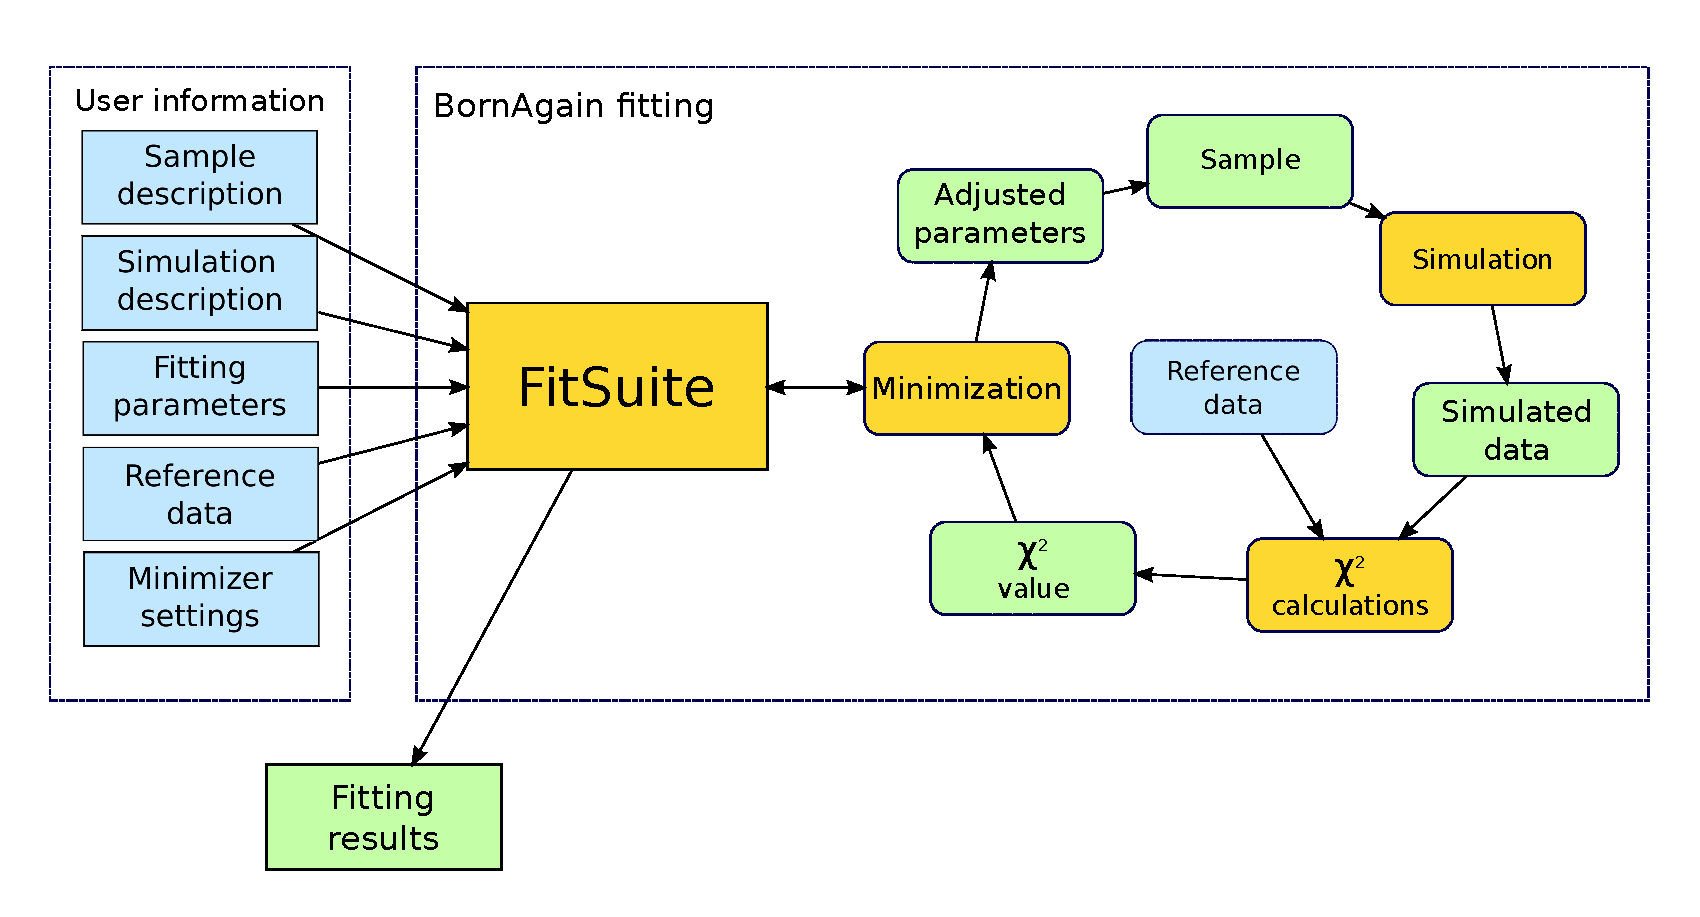
\includegraphics{fig/drawing/minimization_workflow.eps}}
\caption{
Fitting work flow.
}
\label{fig:minimization_workflow}
\end{figure}

Before running the fitting the user is required to prepare some  data and to
configure the fitting kernel of \BornAgain\ . The required stages are

\begin{itemize}
\item Preparing the sample and the simulation description (multilayer, beam, detector parameters).
\item Choosing the fitting parameters.
\item Loading the reference data.
\item Defining the minimization settings.
\end{itemize}

The class \Code{FitSuite} contains the main functionalities to be used for the fit
and serves as the main interface between the user and the fitting work flow. 
The later involves iterations during which

\begin{itemize}
\item The minimizer makes an assumption about the optimal sample parameters.
\item These parameters are propagated to the sample.
\item The simulation is performed for the given state of the sample.
\item The simulated data (intensities) are propagated to the $\chi^2$ module.
\item The later calculates $\chi^2$ using the simulated and reference data.
\item The value of $\chi^2$ is propagated to the minimizer, which makes new assumptions about optimal sample parameters.
\end{itemize}

The iteration process is going on under the control of the selected minimization
algorithm, without any intervention from the
user. It stops 
\begin{itemize}
\item when the maximum number of iteration steps has been exceeded,
\item when the function's minimum has been reached within the tolerance window,
\item if the minimizer could not improve the values of the parameters. 
\end{itemize}

After the control is returned, fitting results can be retrieved.
They consist in the best $\chi^2$ value found, the corresponding
optimal sample parameters and the intensity map simulated with this set of parameters.

%Details of \Code{FitSuite} class implementation and description of each interface are given in \SecRef{FitSuiteClass}. 
The following parts of this section will detail each of
the main stages necessary to run a fitting procedure.


\subsubsection{Preparing the sample and the simulation description}

This step is similar for any simulation using \BornAgain\ (see \SecRef{Simulation}). It consists in first characterizing  the geometry of the system: the particles 
(shapes, sizes, refractive
indices), the different layers (thickness,
order, refractive index, a possible roughness of the interface), the
interference between the particles and the way they are distributed in
the layers (buried particles or particles sitting on top of a
layer). 
Then we specify the parameters of the input beam and of the
output detector.


%===============================================================================
\subsubsection{Choice of parameters to be fitted}
%===============================================================================

In principle, every parameter used in the construction of the sample
can be used as a fitting parameter. For example, the particles'
heights, radii or the layer's roughness or thickness could be selected
using the 
parameter pool mechanism. 
This mechanism is explained in detail in
\SecRef{WorkingWithSampleParameters} and it is therefore recommended
to read it before proceeding any further.

The user specifies selected sample parameters as fit parameters using \Code{FitSuite}
and its \Code{addFitParameter} method
\begin{lstlisting}[language=shell, style=commandline]
fit_suite = FitSuite()
fit_suite.addFitParameter(<name>, <initial value>, <step>, <limits>)
\end{lstlisting}
where \Code{<name>} corresponds to the parameter name in the sample's parameter pool.
By using wildcards in the parameter name, a group of sample parameters, corresponding to the given
pattern, can be associated with a single fitting parameter and 
fitted simultaneously to get a common optimal value (see \SecRef{WorkingWithSampleParameters}).

The second parameter \Code <initial value> correspond to the initial value of
the fitting parameter, while the third one
is responsible to the initial iteration steps size.
The last parameter \Code{<AttLimits>} corresponds to
the boundaries imposed on parameter value. It can be
\begin{itemize}
\item \Code{limitless()} by default, 
\item \Code{fixed()}, 
\item \Code{lowerLimited(<min\_value>)}, 
\item \Code{upperLimited(<max\_value>)}, 
\item \Code{limited(<min\_value>, <max\_value>)}.
\end{itemize}
where \Code{<min\_value>} and \Code{<max\_value>} are
double values corresponding to the lower and higher boundary, respectively.


%===============================================================================
\subsubsection{Associating reference and simulated data}
%===============================================================================

The minimization procedure deals with a pair of reference data (normally
associated with experimental data) and the theoretical model (presented by the sample and the simulation descriptions).

We assume that the experimental data are a two-dimensional intensity 
matrix as function of the output scattering
angles $\alpha_f$ and $\phi_f$ (see Fig.~\ref{fig:multil3d}).
The user is required to provide the data in the form of an ASCII file
containing an axes
binning description and the intensity data itself. 
\vspace*{2mm}

\ImportantPoint{Remark:}{
We recognize the importance of supporting the most common data formats. We are going to provide
this feature in the following releases and welcome users' requests on this subject.
}
\vspace*{1mm}

To associate the simulation and the reference data to the fitting engine, method \newline
\Code{addSimulationAndRealData} has to be used as shown
\begin{lstlisting}[language=python, style=eclipseboxed,numbers=none]
fit_suite = FitSuite()
fit_suite.addSimulationAndRealData(<simulation>, <reference>, <chi2_module>)
\end{lstlisting}

Here \Code{<simulation>} corresponds to a \BornAgain\ simulation object
with the  sample, beam and detector fully defined, \Code{<reference>}
corresponds to the experimental data object obtained from the ASCII file and \Code{<chi2\_module>} is an optional parameter for advanced 
control of $\chi^2$ calculations.

It is possible to call this given method more than once to submit more than one pair of
\Code{<simulation>, <reference>} to the fitting procedure.
In this way, simultaneous fits of
some combined data sets are performed.

By using the third parameter, \Code{<chi2\_module>}, different normalizations and weights
can be applied to give user full control of the way $\chi^2$ is calculated.
This feature will be explained in \SecRef{FittingAdvanced}.


%===============================================================================
\subsection{Minimizer settings}
%===============================================================================

\BornAgain\ contains a variety of minimization engines from \Code{ROOT} and \Code{GSL}
libraries. They are listed in Table~\ref{table:fit_minimizers}.
By default \Code{Minuit2} minimizer with default settings will be used and no additional
configuration needs to be done.
The remainder of this section explains some of the expert settings, which can be applied to get better 
fit results.

The default minimization algorithm can be changed using 
\Code{MinimizerFactory} as shown below
\begin{lstlisting}[language=python, style=eclipseboxed,numbers=none]
fit_suite = FitSuite()
minimizer = MinimizerFactory.createMinimizer("<Minimizer name>","<algorithm>")
fit_suite.setMinimizer(minimizer)
\end{lstlisting}

where \Code{<Minimizer name>} and \Code{<algorithm>} can be chosen from the first and
second column of Table~\ref{table:fit_minimizers} respectively. 
The list of minimization algorithms implemented in \BornAgain\
can also be obtained using \Code{MinimizerFactory.printCatalogue()} command.


\begin{table}[h]
  \small
\centering
\begin{tabular}{@{}lll@{}}
\hline
\hline
\textbf{Minimizer name} & \textbf{Algorithm} & \textbf{Description}\\
\hline
\Code{Minuit2} \cite{MinuitURL} & \Code{Migrad} & According to
\cite{mntutorial} best minimizer for nearly all functions,\\
 & & variable-metric method with inexact line search, \\
 & & a stable metric updating scheme,\\
 & &  and checks for positive-definiteness.\\
\hline
                                       & \Code{Simplex} & simplex method of
                                       Nelder and Mead\\ 
 & & usually slower than \Code{Migrad}, \\
 &  & rather robust with respect to gross fluctuations in the\\ & &  function
 value, gives no reliable information about \\ & &  parameter errors, \\
\hline
                                       & \Code{Combined} & minimization with
                                       \Code{Migrad} \\
                                       & & but switches to Simplex if
                                       Migrad fails to converge.\\
\hline
                                       & \Code{Scan} &  not intended to
                                       minimize, just scans the
                                       function,\\
                                       & &  one parameter at a
                                       time, retains the best value
                                       after\\ &  & each scan\\
\hline
                                       & \Code{Fumili} & optimized
                                       method for least square and log
                                       likelihood\\ & &  minimizations \\
\hline
\Code{GSLMultiMin} \cite{GSLMultiMinURL} & \Code{ConjugateFR} & Fletcher-Reeves conjugate gradient
  algorithm,\\
\hline
& \Code{ConjugatePR} & Polak-Ribiere conjugate gradient algorithm,\\ 
\hline
& \Code{BFGS} & Broyden-Fletcher-Goldfarb-Shanno algorithm,\\ 
\hline
& \Code{BFGS2} & improved version of BFGS,\\ 
\hline
& \Code{SteepestDescent} & follows the downhill gradient of the function at each step\\
\hline
\Code{GSLLMA} \cite{GSLMultiFitURL} & & Levenberg-Marquardt
Algorithm\\
\hline
\Code{GSLSimAn} \cite{GSLSimAnURL}& & Simulated Annealing Algorithm\\ 
\hline
\hline
\end{tabular}
\caption{List of minimizers implemented in \BornAgain. }
\label{table:fit_minimizers}
\index{Minimizers}
\end{table}

There are several options common to every minimization algorithm, which can be changed
before starting the minimization. They are handled by \Code{MinimizerOptions} class:
\begin{lstlisting}[language=python, style=eclipseboxed, numbers = none]
fit_suite.getMinimizer().getOptions().setMaxFunctionCalls(10)
\end{lstlisting}
In the above code snippet, a number of ``maximum function calls'',
namely the maximum number of times the minimizer is allowed to call the simulation, is limited to 10. %The minimizer will take that number into consideration and will try to limit number of iterations by that value.

There are also expert-level options common for all minimizers as well
as a number of options to tune individual minimization algorithms.
They will be explained in \SecRef{FittingAdvanced}.


%===============================================================================
\subsection{Running the fitting ant retrieving the results}
%===============================================================================

After the initial configuration of \Code{FitSuite} has been performed, the fitting
can be started using the command
\begin{lstlisting}[language=python, style=eclipseboxed, numbers = none]
fit_suite.runFit()
\end{lstlisting}

Depending on the complexity of the sample and the number of free sample parameters the fitting
process can take from tens to thousands of iterations. The results of the fit can
be printed on the screen using the command
\begin{lstlisting}[language=python, style=eclipseboxed, numbers = none]
fit_suite.printResults()
\end{lstlisting}
\SecRef{FittingExamples} gives more details about how to access the fitting results.


%===============================================================================
\subsection{Basic Python fitting example} \SecLabel{FittingExamples}
%===============================================================================

In this section we are going to go through a complete example of
fitting using \BornAgain. Each  step will be associated with a
detailed piece of code written in \Python. 
The complete listing of
the script is given in Appendix (see Listing~\ref{PythonFittingExampleScript}).
The script can also be found at
\begin{lstlisting}[language=shell, style=commandline]
./Examples/python/fitting/ex002_FitCylindersAndPrisms/FitCylindersAndPrisms.py
\end{lstlisting}

\noindent
This example uses the same sample geometry as in \SecRef{Example1Python}.
Cylindrical and
prismatic particles in equal proportion are deposited on a substrate layer, with no interference
between the particles. We consider the following parameters to be unkown
\begin{itemize}
\item the radius of cylinders,
\item the height of cylinders,
\item the length of the prisms' triangular basis,
\item the height of prisms.
\end{itemize}

Our reference data are a ``noisy'' two-dimensional intensity
map obtained from the simulation of the same geometry with a fixed
value of $5\,{\rm nm}$ for the height and radius of cylinders and for the
height of prisms which have a 10-nanometer-long side length. 
Then we run our fitting using default minimizer settings
starting with a cylinder's height
of $4\,{\rm nm}$, a cylinder's radius of $6\,{\rm nm}$, 
a prism's half side of $6\,{\rm nm}$ and a height equal to $4\,{\rm nm}$.
As a result, the fitting procedure is able to find the correct value of $5\,{\rm nm}$
for all four parameters.


%-------------------------------------------------------------------------------
\subsubsection*{Importing Python libraries}
%-------------------------------------------------------------------------------

\begin{lstlisting}[language=python, style=eclipseboxed]
from libBornAgainCore import *
from libBornAgainFit import *
\end{lstlisting}
We start from importing two \BornAgain\ libraries required to create
the sample description
and to run the fitting.

%-------------------------------------------------------------------------------
\subsubsection*{Building the sample}
%-------------------------------------------------------------------------------

\begin{lstlisting}[language=python, style=eclipseboxed, firstnumber=5]
def get_sample(): @\label{script2::get_sample}@
    """
    Build the sample representing cylinders and pyramids on top of substrate without interference.
    """
    # defining materials
    m_air = HomogeneousMaterial("Air", 0.0, 0.0)
    m_substrate = HomogeneousMaterial("Substrate", 6e-6, 2e-8)
    m_particle = HomogeneousMaterial("Particle", 6e-4, 2e-8)

    # collection of particles
    cylinder_ff = FormFactorCylinder(1.0*nanometer, 1.0*nanometer)
    cylinder = Particle(m_particle, cylinder_ff)
    prism_ff = FormFactorPrism3(2.0*nanometer, 1.0*nanometer)
    prism = Particle(m_particle, prism_ff)
    particle_layout = ParticleLayout()
    particle_layout.addParticle(cylinder, 0.0, 0.5)
    particle_layout.addParticle(prism, 0.0, 0.5)
    interference = InterferenceFunctionNone()
    particle_layout.addInterferenceFunction(interference)

    # air layer with particles and substrate form multi layer
    air_layer = Layer(m_air)
    air_layer.addLayout(particle_layout)
    substrate_layer = Layer(m_substrate)
    multi_layer = MultiLayer()
    multi_layer.addLayer(air_layer)
    multi_layer.addLayer(substrate_layer)
    return multi_layer
\end{lstlisting}
The function starting at line~\ref{script2::get_sample} creates a multilayered sample
with cylinders and prisms using arbitrary $1\,{\rm nm}$ value for all size's of particles.
The details about the generation of this multilayered sample are given in \SecRef{Example1Python}.

%-------------------------------------------------------------------------------
\subsubsection*{Creating the simulation}
%-------------------------------------------------------------------------------
\begin{lstlisting}[language=python, style=eclipseboxed, firstnumber=35]
def get_simulation(): @\label{script2::get_simulation}@
    """
    Create GISAXS simulation with beam and detector defined
    """
    simulation = Simulation()
    simulation.setDetectorParameters(100, -1.0*degree, 1.0*degree, 100, 0.0*degree, 2.0*degree)
    simulation.setBeamParameters(1.0*angstrom, 0.2*degree, 0.0*degree)
    return simulation
\end{lstlisting}
The function starting at line~\ref{script2::get_simulation} creates
the simulation object with the definition of the beam and detector parameters.

%-------------------------------------------------------------------------------
\subsubsection*{Preparing the fitting pair}
%-------------------------------------------------------------------------------
\begin{lstlisting}[language=python, style=eclipseboxed, firstnumber=45]
def run_fitting(): @\label{script2::run_fitting}@
    """
    run fitting
    """
    sample = get_sample() @\label{script2::setup_simulation1}@
    simulation = get_simulation()
    simulation.setSample(sample) @\label{script2::setup_simulation2}@

    real_data = IntensityDataIOFactory.readIntensityData('refdata_fitcylinderprisms.int.gz') @\label{script2::real_data}@
\end{lstlisting}
Lines
~\ref{script2::setup_simulation1}-~\ref{script2::setup_simulation2}
generate the 
sample and simulation description and assign the sample to the simulation.
Our reference data are contained in the file \Code{'refdata\_fitcylinderprisms.int.gz'}.
 This reference had been generated by adding noise
on the scattered intensity from a numerical sample with a fixed length of 5~nm for the four fitting
parameters (\textit{i.e.} the dimensions of the cylinders and prisms).
Line ~\ref{script2::real_data} creates the real data object by loading
the ASCII data from the input file.

%-------------------------------------------------------------------------------
\subsubsection*{Setting up \rm\bf{FitSuite}}
%-------------------------------------------------------------------------------
\begin{lstlisting}[language=python, style=eclipseboxed, firstnumber=55]
    fit_suite = FitSuite() @\label{script2::fitsuite1}@
    fit_suite.addSimulationAndRealData(simulation, real_data) @\label{script2::fitsuite2}@
    fit_suite.initPrint(10) @\label{script2::fitsuite3}@
\end{lstlisting}
Line ~\ref{script2::fitsuite1} creates a \Code{FitSuite} object which provides
the main interface to the minimization kernel of \BornAgain\ . 
Line ~\ref{script2::fitsuite2} submits simulation description and real data pair to the 
subsequent fitting. Line ~\ref{script2::fitsuite3} sets up \Code{FitSuite} to print on
the screen the information about fit progress once per 10 iterations.
\begin{lstlisting}[language=python, style=eclipseboxed, firstnumber=60]
    fit_suite.addFitParameter("*FormFactorCylinder/height", 4.*nanometer, 0.01*nanometer, AttLimits.lowerLimited(0.01)) @\label{script2::fitpars1}@
    fit_suite.addFitParameter("*FormFactorCylinder/radius", 6.*nanometer, 0.01*nanometer, AttLimits.lowerLimited(0.01))
    fit_suite.addFitParameter("*FormFactorPrism3/height", 4.*nanometer, 0.01*nanometer, AttLimits.lowerLimited(0.01))
    fit_suite.addFitParameter("*FormFactorPrism3/length", 12.*nanometer, 0.02*nanometer, AttLimits.lowerLimited(0.01)) @\label{script2::fitpars2}@
\end{lstlisting}
Lines ~\ref{script2::fitpars1}--~\ref{script2::fitpars2} enter the
list of fitting parameters. Here we use the cylinders' height and
radius and the prisms' height and side length. 
The cylinder's length and prism half side are initially equal to $4\,{\rm nm}$,
whereas the cylinder's radius and the prism half side length are equal to $6\,{\rm nm}$ before the minimization. The
iteration step is equal to $0.01\,{\rm nm}$ and only the lower
boundary is imposed to be equal to $0.01\,{\rm nm}$.

%-------------------------------------------------------------------------------
\subsubsection*{Running the fit and accessing results}
%-------------------------------------------------------------------------------
\begin{lstlisting}[language=python, style=eclipseboxed, firstnumber=66]
    fit_suite.runFit() @\label{script2::fitresults1}@

    print "Fitting completed."
    fit_suite.printResults()@\label{script2::fitresults2}@
    print "chi2:", fit_suite.getMinimizer().getMinValue() 
    fitpars = fit_suite.getFitParameters()
    for i in range(0, fitpars.size()):
        print fitpars[i].getName(), fitpars[i].getValue(), fitpars[i].getError() @\label{script2::fitresults3}@
\end{lstlisting}
Line ~\ref{script2::fitresults1} shows the command to start the fitting process.
During the fitting the progress will be displayed on the screen.
Lines ~\ref{script2::fitresults2}--~\ref{script2::fitresults3} shows different ways of
accessing the fit results.


More details about fitting, access to its results and visualization of
the fit progress using matplotlib libraries can be learned from the
following detailed example
\begin{lstlisting}[language=shell, style=commandline]
./Examples/python/fitting/ex002_FitCylindersAndPrisms/FitCylindersAndPrisms_detailed.py
\end{lstlisting}


%===============================================================================
\subsection {Advanced fitting} \SecLabel{FittingAdvanced}
%===============================================================================

\subsubsection{Affecting $\chi2$ calculations}
\subsubsection{Simultaneous fits of several data sets}
\subsubsection{Using fitting strategies}
\subsubsection{Masking the real data}
\subsubsection{Tuning fitting algorithms}
\subsubsection{Fitting with correlated sample parameters}


%===============================================================================
\subsection {How to get the right answer from fitting}
  \SecLabel{FittingRightAnswers}
%===============================================================================

%As it has already been mentioned in \SecRef{FittingGentleIntroducion}, 
One of the main difficulties in fitting the data with the model 
is the presence of multiple
local minima in the objective function. Many problems can cause the
fit to fail, for example:
\begin{itemize}
\item an unreliable physical model,
\item an unappropriate choice of objective function
\item multiple local minima,
\item an unphysical behavior of the objective function, unphysical regions
  in the parameters space,
\item an unreliable parameter error calculation in the presence of
  limits on the parameter value,
\item an exponential behavior of the objective function and the
  corresponding numerical inaccuracies, excessive numerical roundoff
  in the calculation of its value and derivatives,
\item large correlations between parameters,
\item very different scales of parameters involved in the calculation,
\item not positive definite error matrix even at minimum.
\end{itemize}


The given list, of course, is not only related to \BornAgain\
fitting. It remains applicable to any fitting program and any kind of theoretical model.
%To address all these difficulties some amount of manual tuning might be necessary.
 Below we give some recommendations which might help the user to achieve reliable fit results.

\subsection*{General recommendations}
\begin{itemize}
\item initially choose  a small number of free fitting parameters,
\item eliminate redundant parameters,
\item provide a good initial guess for the fit parameters,
\item start from the default minimizer settings and perform some fine tuning after some experience has been acquired,
\item repeat the fit using different starting values for the parameters or their limits,
\item repeat the fit, fixing and varying different groups of parameters,
%\item use \Code{Minuit2} minimizer with \Code{Migrad} algorithm
%  (default) to get the most reliable parameter error estimation,
%\item try \Code{GSLMultiFit} minimizer or \Code{Minuit2} minimizer with \Code{Fumili} %algorithm to get fewer iterations.


%\subsection*{Interpretation of errors.}


{\bf to be continued... }


\end{itemize}

\index{Fitting|)}

%%%%%%%%%%%%%%%%%%%%%%%%%%%%%%%%%%%%%%%%%%%%%%%%%%%%%%%%%%%%%%%%%%%%%%%%%%%%%%%%
\section{User API} \label{UserAPI}
%%%%%%%%%%%%%%%%%%%%%%%%%%%%%%%%%%%%%%%%%%%%%%%%%%%%%%%%%%%%%%%%%%%%%%%%%%%%%%%%

%===============================================================================
\subsection{IntensityData}
%===============================================================================

The \Code{IntensityData} object stores the 
simulated or real intensity data together with the axes definition of the detector in BornAgain's internal format. 
During the simulation setup
it is created automatically when the user specifies the detector characteristics and is filled with the simulated intensities after the simulation is completed.

\begin{lstlisting}[language=python, style=eclipseboxed]
simulation = Simulation()
simulation.setDetectorParameters(10, -5.0*degree, 5.0*degree, 5, 0.0*degree, 1.0*degree)
...
simulation.runSimulation()
intensity = simulation.getIntensityData() @\label{py:UserApi:intensity}@
\end{lstlisting}

The \Code{IntensityData} object retrieved in line~\ref{py:UserApi:intensity} corresponds to
the two dimensional detector pixel array as shown in Fig.~\ref{fig:UserApi:IntensityData}.

\begin{figure}[ht]
  \centering
    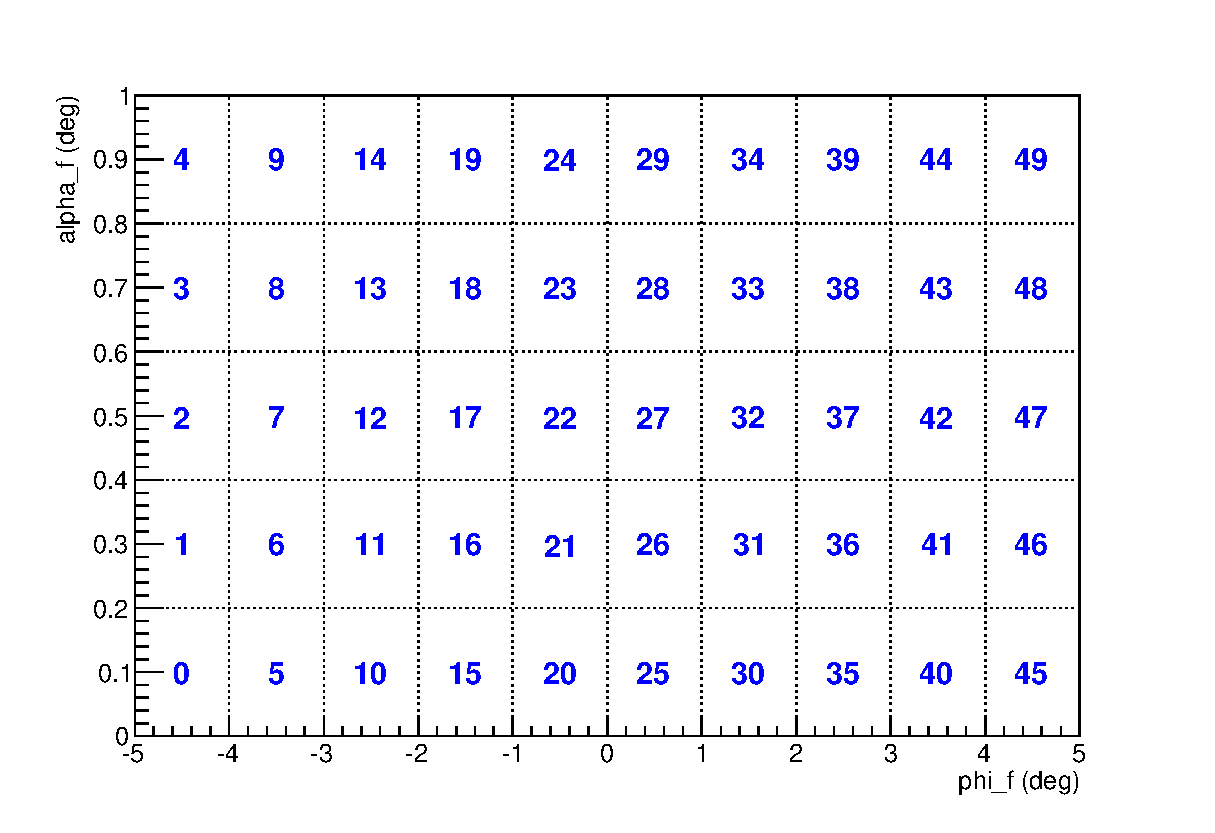
\includegraphics[clip=, width=120mm]{fig/drawing/UserAPI_IntensityDataLayout.eps}
  \caption{The axes layout of IntensityData object.}
  \label{fig:UserApi:IntensityData}
\end{figure}

The x-axis and y-axis of the figure correspond to the $\phi_f$ and $\alpha_f$ axes of the detector. 
The x-axis is divided into 10 bins,
with low edge of the first bin set to $-5.0\,{\rm deg}$ and upper edge of the last bin set to $+5.0\,{\rm deg}$.
The y-axis is divided into 5 bins,
with low edge of the first bin set to $0.0\,{\rm deg}$ and upper edge of the last bin set to $1.0\,{\rm deg}$.
There are 50 bins in total (they are marked on the plot with indexes from 0 to 49), each bin will contain one intensity value.

During a standard simulation (i.e. no Monte-Carlo integration involved) intensities are calculated for $\phi_f, \alpha_f$ values corresponding to the bin centers, e.g. the intensity stored in bin\#42 will correspond to $\phi_f=3.5\,{\rm deg}, \alpha_f=0.5\,{\rm deg}$. 
\vspace*{2mm}


\MakeRemark{}{
The \Code{IntensityData} object is not intended for direct usage from Python API. The idea is 
that the API provides the user with the possibility to export the data from BornAgain internal format to the format of his choice as well as import user's data into BornAgain.
For the moment this functionality is limited to a few options explained below.
We encourage users feedback to implement the support of most requested formats.
}\\



\subsubsection{Import/export of intensity data}
For the moment we provide following options:
\begin{itemize}
\item Import/export of \Code{IntensityData} object from/to \Code{numpy} array.
\item Import/export of \Code{IntensityData} object from/to text file.

\end{itemize}

\paragraph{Export to numpy array}

To export intensity data into  \Code{numpy} array the method \Code{getArray()} should be used 
on \Code{IntensityData} object as shown in line \ref{py:UserApi:getArray} of
following code snippet.

\begin{lstlisting}[language=python, style=eclipseboxed]
intensity = simulation.getIntensityData()
array = intensity.getArray() @\label{py:UserApi:getArray}@
...
pylab.imshow(numpy.rot90(array, 1)) @\label{py:UserApi:imshow}@
pylab.show()
\end{lstlisting}

For the detector settings defined in the previous paragraph the dimensions of the resulting array will be (10,5). By using \Code{numpy} indexes the user can get access to the intensity values, e.g.
\Code{array[0][0]} corresponds to the intensity in bin\#0 of Fig.~\ref{fig:UserApi:IntensityData},
\Code{array[0][4]} to bin\#4, 
\Code{array[1][0]} to bin\#5, 
\Code{array[8][2]} to bin\#42, 
\Code{array[9][4]} to bin\#49. 


To plot this resulting numpy array with \Code{matplotlib} it has to be rotated counter-clockwise
to match \Code{matplotlib} conventions as shown in line~\ref{py:UserApi:imshow}.


%\subsubsection{Direct access to the data}
%User can access to the

%\begin{lstlisting}[language=python, style=eclipseboxed]
%for i in range(0, intensity.getAllocatedSize()):
%    print intensity[i]
%\end{lstlisting}


\subsubsection{Importing from numpy array}

To use fitting the user has to load experimental data into BornAgain fitting kernel.
To read experimental data the user has to create
IntensityData object, fill it with the experimental  intensity values and pass
this object to the fitting kernel.

First, the user creates empty \Code{IntensityData} as shown
in line~\ref{py:UserApi:IntensityData} of the following code snippet.
\begin{lstlisting}[language=python, style=eclipseboxed]
data = IntensityData() @\label{py:UserApi:IntensityData}@
data.addAxis(FixedBinAxis("phi_f", 10, -5.0*degree, 5.0*degree)) @\label{py:UserApi:phi_f}@
data.addAxis(FixedBinAxis("alpha_f", 5, 0.0*degree, 1.0*degree)) @\label{py:UserApi:alpha_f}@
...
array = numpy.zeros((10, 5)) # fill array with experimental intensities @\label{py:UserApi:create_array}@
...
data.setRawDataVector(array.flatten().tolist()) @\label{py:UserApi:set_raw}@

fitSuite = FitSuite() @\label{py:UserApi:fit_suite}@
fitSuite.addSimulationAndRealData(simulation, data) @\label{py:UserApi:add_real_data}@
\end{lstlisting}

In lines~\ref{py:UserApi:phi_f}, \ref{py:UserApi:alpha_f} two axes with fixed bin sizes
are defined to represent the detector layout as shown in Fig.~\ref{fig:UserApi:IntensityData}. 
The constructor of \Code{FixedBinAxis} object has the following signature

\begin{lstlisting}[language=python, style=eclipse,numbers=none]
FixedBinAxis(title, nbins, min_angle, max_angle)
\end{lstlisting}

The created \Code{IntensityData} object has to be filled with experimental intensities
using \Code{numpy} array prepared by the user (lines ~\ref{py:UserApi:create_array}-~\ref{py:UserApi:set_raw}). In lines \ref{py:UserApi:fit_suite},\ref{py:UserApi:add_real_data} the fitting kernel is created and initialized with \Code{Simulation} object and 
\Code{IntensityData} object representing the experimental data.


\subsubsection{Saving intensity data to text file.}

The special class \Code{IntensityDataIOFactory} is intended for saving the intensity data
in different datafile formats. For the moment, it only supports saving the data in specific BornAgain's text files (the file extention \Code{*.int}).

\begin{lstlisting}[language=python, style=eclipseboxed]
intensity = simulation.getIntensityData()
IntensityDataIOFactory.writeIntensityData(intensity, 'file_name.int')
\end{lstlisting}

\subsubsection{Reading intensity data from a text file.}
The same class is also intended for reading intensity data
from files with different formats. For the moment, it only supports reading the data from text files of special BornAgain's format (the file extention \Code{*.int}).
 
\begin{lstlisting}[language=python, style=eclipseboxed]
intensity = IntensityDataIOFactory.readIntensityData('file_name.int')
\end{lstlisting}
